% reviewers: schatz, pop, durbin, pevzner.

% @@add commentary on trinity table / k-mer loss.
% @@spellcheck!
% @graph of k-mer count vs data
%
% @schizo mapping coverage graph for mrnaseq?
% @error correction could be applied at C=20 stage to mrnaseq
% @long reads!
% @error correction after diginorm <=> skewed abundance dists.

% Template for PLoS
% Version 1.0 January 2009
%
% To compile to pdf, run:
% latex plos.template
% bibtex plos.template
% latex plos.template
% latex plos.template
% dvipdf plos.template

\documentclass[10pt]{article}

% amsmath package, useful for mathematical formulas
\usepackage{amsmath}
% amssymb package, useful for mathematical symbols
\usepackage{amssymb}

% graphicx package, useful for including eps and pdf graphics
% include graphics with the command \includegraphics
\usepackage{graphicx}

% cite package, to clean up citations in the main text. Do not remove.
\usepackage{cite}

\usepackage{color} 

% Use doublespacing - comment out for single spacing
%\usepackage{setspace} 
%\doublespacing


% Text layout
\topmargin 0.0cm
\oddsidemargin 0.5cm
\evensidemargin 0.5cm
\textwidth 16cm 
\textheight 21cm

% Bold the 'Figure #' in the caption and separate it with a period
% Captions will be left justified
\usepackage[labelfont=bf,labelsep=period,justification=raggedright]{caption}

% Use the PLoS provided bibtex style
\bibliographystyle{plos2009}

% Remove brackets from numbering in List of References
\makeatletter
\renewcommand{\@biblabel}[1]{\quad#1.}
\makeatother


% Leave date blank
\date{}

\pagestyle{myheadings}
%% ** EDIT HERE **


%% ** EDIT HERE **
%% PLEASE INCLUDE ALL MACROS BELOW

%% END MACROS SECTION

\begin{document}

% Title must be 150 characters or less
\begin{flushleft}
{\Large
\textbf{A single pass approach to reducing sampling variation, removing
errors, and scaling {\em de novo} assembly of shotgun sequences}}
% Insert Author names, affiliations and corresponding author email.
\\
C. Titus Brown$^{1,\ast}$, 
Adina Howe$^{2}$,
Qingpeng Zhang$^{3}$,
Alexis B. Pyrkosz$^{4}$,
Timothy H. Brom$^{3}$
\\
\bf{1} Departments of Computer Science and Engineering/Microbiology and Molecular Genetics, Michigan State University, East Lansing, MI, USA
\\
\bf{2} Departments of Microbiology and Molecular Genetics/Crop and Soil Sciences, Michigan State University, East Lansing, MI, USA
\\
\bf{3} Department of Computer Science and Engineering, Michigan State University, East Lansing, MI, USA
\\
{\bf{4} USDA Avian Disease and Oncology Laboratory, East Lansing, MI, USA}
\\
$\ast$ E-mail: Corresponding ctb@msu.edu
\end{flushleft}

% Please keep the abstract between 250 and 300 words
\section*{Abstract}

{\bf Background:} Deep shotgun sequencing and analysis of genomes,
transcriptomes, amplified single-cell genomes, and metagenomes enable
the sensitive investigation of a wide range of biological
phenomena. However, it is increasingly difficult to deal with the
volume of data emerging from deep short-read sequencers, in part
because of random and systematic sampling variation as well as a high
sequencing error rate.  These challenges have led to the development of
entire new classes of short-read mapping tools, as well as new {\em de novo}
assemblers.  Even newer assembly strategies for dealing with
transcriptomes, single-cell genomes, and metagenomes have also
emerged.  Despite these advances, algorithms and compute capacity
continue to be challenged by the continued improvements in sequencing
technology throughput.
\\
\\
{\bf Methodology and Principal Findings:} We describe an approach we term
digital normalization, a single-pass computational algorithm that
discards redundant data and both sampling variation and the number of errors
present in deep sequencing data sets. Digital normalization substantially
reduces the size of data sets and accordingly decreases the memory and time
requirements for {\em de novo} sequence assembly, all without significantly
impacting content of the generated contigs.  In doing so, it converts
high random coverage to low systematic coverage.
\\
\\
{\bf Conclusions and Significance:} Digital normalization is an
effective and efficient approach to normalizing coverage, removing errors,
and reducing data set size for shotgun sequencing data sets.
It is particularly useful for reducing the compute requirements for
{\em de novo} sequence assembly.  We demonstrate this for the assembly
of microbial genomes, amplified single-cell genomic data, and
transcriptomic data.  The software is freely available for use and
modification.

% Please keep the Author Summary between 150 and 200 words
% Use first person. PLoS ONE authors please skip this step. 
% Author Summary not valid for PLoS ONE submissions.   
\section*{Author Summary}

\section*{Introduction}

The ongoing improvements in DNA sequencing technologies have led to a new
problem: how do we analyze the resulting large sequence data sets
quickly and efficiently? These data sets contain millions to billions
of short reads, and have high error rates and substantial sampling
biases \cite{pubmed19997069}.  The vast quantities of deep sequencing data produced by
these new sequencing technologies are driving
computational biology to extend and adapt previous approaches to sequence
analysis.  In
particular, the widespread use of deep shotgun sequencing on
previously unsequenced genomes, transcriptomes, and metagenomes, has
resulted in the development of several new approaches to {\em de novo}
sequence assembly \cite{pubmed20211242}.

There are two basic challenges in analyzing short-read sequences from
shotgun sequencing. First, deep sequencing is needed for complete
sampling. This is because shotgun sequencing samples randomly from the
population of molecules; this sampling is biased by sample content and
sample preparation, requiring even deeper sequencing. A human genome
may require 100x coverage or more for near-complete sampling, leading
to shotgun data sets 100 or more times the size of the human genome
\cite{pubmed21187386}.  Since the lowest abundance molecule determines
the depth of coverage required for complete sampling, transcriptomes
and metagenomes containing rare transcripts and genomes can also
require similarly deep sequencing.  Thus many shotgun data sets are
also quite large.

The second challenge to analyzing short-read shotgun sequencing is the
high error rate.  For example, the Illumina GAII has a 1-2\% error
rate, yielding an average of one base error in every 100 bp of data
\cite{pubmed19997069}.  The total number of errors grows linearly with
the amount of data generated, so these errors usually dominate
novelty in large data sets \cite{pubmed21245053}.  Tracking this
novelty and resolving errors is computationally expensive.

These large data sets and high error rates combine to provide a third
challenge: it is now straightforward to generate data sets that cannot
easily be analyzed \cite{pubmed21867570}.  While hardware approaches
to scaling existing algorithms are emerging, sequencing capacity
continues to grow faster than computational capacity
\cite{pubmed20441614}.  Therefore, new algorithmic approaches to
analysis are needed.

Many new algorithms and tools have been developed to tackle large and
error-prone short-read shotgun data sets. A new class of alignment
tools, mostly relying on the Burrows-Wheeler transform, has been
created specifically to do ultra-fast short-read alignment to
reference sequence \cite{pubmed19430453}.  In cases where a reference
sequence does not exist and must be assembled {\em de novo} from the
sequence data, a number of new assemblers have been written, including
ABySS, Velvet, SOAPdenovo, ALLPATHS, and SGA
\cite{pubmed20211242,pubmed21187386,pubmed22156294}.  These assemblers
rely on theoretical advances, including de Bruijn graphs and
FM-indices, to store and traverse large amounts of data
\cite{pubmed22068540,pubmed20529929}.  As short-read sequencing has
been applied to single cell genomes, transcriptomes, and metagenomes,
yet another generation of assemblers has emerged to handle reads from
abundance-skewed populations of molecules; these tools, including
Trinity, Oases, MetaVelvet, Meta-IDBA, and Velvet-SC, adopt local
models of sequence coverage to help build assemblies
\cite{pubmed21572440,pubmed22368243,metavelvet,pubmed21685107,pubmed21926975}.
Because these tools all rely on k-mer approaches and require exact
matches to construct overlaps between sequences, their performance is
very sensitive to the number of errors present in the underlying data.
This sensitivity to errors has led to the development of a number of
error removal and correction approaches that preprocess data prior to
assembly or mapping
\cite{pubmed21685062,pubmed15059830,pubmed21114842}.

One approach to error correction involves finding low-abundance
fixed-length words, or k-mers, and treating them as likely errors;
these errors can then be ``corrected'' by changing them to similar
k-mers that are in high abundance \cite{pubmed21114842}.  This
approach requires two complete iterations across the data set: one
iteration to collect abundance spectra, and a second to perform the
trimming or correction.  For extremely large data sets, this is a
significant problem: the ``noise'' from sequencing errors drives a
supra-linear increase in the number of k-mers, so as data set size
increases, the computation and memory needed to track k-mers increases
dramatically \cite{pubmed21245053}.


Below, we introduce ``digital normalization'', a single-pass algorithm
for elimination of redundant reads in data sets.  Digital
normalization is inspired by experimental normalization techniques
developed for cDNA library preparation, in which hybridization
kinetics are exploited to reduce the copy number of abundant
transcripts prior to sequencing\cite{pubmed8889548,pubmed7937745}.
{\em Digital} normalization works after sequencing data has been
generated, progressively removing high-coverage reads from shotgun
data sets.  This normalizes average coverage to a specified value,
reducing sampling variation while removing reads and errors contained
within discarded reads.  The data and error reduction results in
decreased computational requirements for {\em de novo} assembly.

%The digital normalization algorithm is inspired by experimental
%normalization techniques developed for cDNA library preparation.  In
%experimental normalization, hybridization kinetics are exploited to
%reduce the copy number of highly abundant transcripts, ``normalizing''
%or evening out the abundance distribution so that shotgun cloning and
%sequencing recover low-abundance molecules as well as high-abundance
%molecules \cite{pubmed8889548,pubmed7937745}.  {\em Digital}
%normalization was initially designed to deal with reads from
%abundance-skewed samples such as single-cell amplified genomic DNA,
%transcriptomes, and metagenomes
%\cite{pubmed16732271,pubmed19015660,pubmed16304596}.

%Digital normalization systematically removes high-coverage reads from
%data sets.  Errors contained in these discarded reads do not then
%accumulate in the normalized data set, and we see a substantial
%reduction in the total number of errors.

We present a fixed-memory implementation of digital normalization that
operates in time linear with the size of the input data.  We then
demonstrate its effectiveness for reducing compute requirements for
{\em de novo} assembly on several real data sets.  These data sets
include an {\em E. coli} genomic data set, two single-cell microbial
genomes, and yeast and mouse mRNAseq samples.

% Results and Discussion can be combined.
\section*{Results}

\subsection*{Estimating sequencing depth without a reference assembly}

Short-read assembly requires deep sequencing to systematically sample
the source genome, because shotgun sequencing is subject to both
random sampling variation and systematic sequencing biases.  For
example, 100x sampling of a human genome is required for recovery of
90\% or more of the genome in contigs $>$ 1kb \cite{pubmed21187386}.
In principle much of this high-coverage data is redundant and could be
eliminated without consequence to the final assembly, but determining
which reads to eliminate requires a per-read estimate of coverage.
Traditional approaches estimate coverage by mapping reads to an
assembly.  This presents a chicken-and-egg problem: in order to
determine which regions are oversampled, we must already have an
assembly!

We may calculate a {\em reference-free} estimate of genome coverage by
looking at the k-mer abundance distribution within individual reads.
First, observe that k-mers, DNA words of a fixed length $k$, tend to
have similar abundances within a read: this is a well-known property
of k-mers that stems from each read coming from a single source
molecule of DNA.  The more times a region is sequenced, the higher the
abundance of k-mers from that region would be.  In the absence of
errors, then, the average k-mer abundance could be used as an estimate
of the depth of coverage for a particular read (Figure
\ref{fig:rankabund}, ``no errors'' line).  However, when reads contain
random substitution or indel errors from sequencing, the k-mers
containing these errors will be of lower abundance; this feature is
often used in k-mer based error correction approaches
\cite{pubmed21114842}.  A single substitution will introduce $k$
low-abundance k-mers within a read.  (Figure \ref{fig:rankabund},
``single substitution error'' line).  However, for small $k$ and reads
of length $L$, a single substitution error will not skew the {\em
  median} k-mer abundance; in fact, as long as $L > 3k-1$, the median
k-mer abundance will be insensitive to a single error.  Only when
multiple substitution errors are found in a single read will the
median k-mer abundance be affected (Figure \ref{fig:rankabund},
``multiple substitution errors'').

Using a fixed-memory CountMin Sketch data structure to count k-mers
(see Methods and \cite{countminsketch}), we see that median k-mer
abundance correlates well with mapping-based coverage for artificial
and real genomic data sets.  Figure \ref{fig:random} shows a strong
correlation between median k-mer abundance and mapping-based coverage
both for simulated 100-base reads generated with 1\% error from a
400kb artificial genome sequence (Figure \ref{fig:random}a, $r^2 =
0.79$), as well as for real short-read data from {\em E. coli} (Figure
\ref{fig:random}b, $r^2 = 0.80$).  In Figure \ref{fig:transcripts}, we
see that the correlation between median k-mer abundance and
mapping-based coverage also holds for abundance-skewed data, both
simulated (Figure \ref{fig:transcripts}a, $r^2 = 0.93$) and real mouse
transcriptome data (Figure \ref{fig:transcripts}b, $r^2 = 0.90$); note
log-log axes.  Points that lie above the $x=y$ line represent reads
that contain high-abundance k-mers that skew the median k-mer
abundance upwards, while reads below the $x=y$ line represent reads
with many errors.  These error-containing reads can still be
accurately mapped, but the errors interfere with the median k-mer
abundance.

Thus we can see that the median k-mer abundance of a read correlates
well with mapping-based estimates of read coverage.
We next investigate ways of using this estimator to remove highly
sampled regions prior to {\em de novo} assembly.

\subsection*{Eliminating redundant reads reduces variation in sequencing depth}

Deeply sequenced genomes will contain many highly covered loci.  For
example, in a human genome sequenced to 100x average coverage, we would
expect 50\% or more of the reads to have a coverage greater than 100.
In practice, we should need only a few of these reads to actually assemble
the source locus.

Using the median k-mer abundance estimator, we can examine each read
in the data set progressively to determine if it is high coverage.  At
the beginning of a shotgun data set, we would expect many reads to be
entirely novel and have a low estimated coverage; as we proceed
through the data set, however, average coverage will increase and many
reads will be from loci for which we already have many reads.

Suppose we choose a coverage threshold $C$ past which we no longer
wish to collect reads. If we only keep reads whose estimated coverage
is less than $C$, and discard the rest, we will reduce the average
coverage of the data set below $C$.  This procedure is
algorithmically straightforward to execute: we examine each read's
estimated coverage, and retain only those whose coverage is less than $C$.
The following pseudocode provides one approach:
\begin{verbatim}
   for read in dataset:
      if estimated_coverage(read) < C:
         accept(read)
      else:
         discard(read)
\end{verbatim}
\noindent
where accepted reads contribute to the $\tt estimated\_coverage$
function.  Note that for any data set with an average coverage $> 2C$,
this has the effect of discarding the majority of reads.  Critically,
low-coverage reads, especially reads from undersampled regions, will
always be retained.

The net effect of this procedure, which we call digital normalization,
is to shift the coverage distribution of data sets to the left, while
systematically subsampling the coverage.  In Figure
\ref{fig:coverage}, we display the estimated coverage of both a
simulated genome and an {\em E. coli} genome for both pre- and
post-normalization data sets, using read multimapping.  From this, we
see that digital normalization has the predicted effect of
systematically shifting the estimated coverage of the reads; since the
median k-mer abundance is generally lower than the coverage (Figures
\ref{fig:rankabund}, \ref{fig:random}, and \ref{fig:transcripts}), the
new average mapping coverage is higher than C.  We also note that
digital normalization has the effect of reducing high random sampling
to more systematic sampling at lower coverage.

At what rate are sequences retained?  For the {\em E. coli} data set,
Figure \ref{fig:accumulate} shows the fraction of sequences retained
by digital normalization as a function of the total number of reads
examined when normalizing to C=20 at k=20.  There is a clear
saturation effect showing that as more reads are examined, a smaller
fraction of reads is retained; by 5m reads, approximately 50-100x
coverage of {\em E. coli}, under 30\% of new reads are kept.  This
demonstrates that as expected, only a small amount of novelty (in
the form of either new information, or the systematic accumulation of
errors) is being observed with increasing sequencing depth.

% @CTB figure 4b / transcriptome/mouse stuff?

\subsection*{Digital normalization retains information while discarding
both data and errors}

The per-base error rate of most next-generation sequencing
technologies approaches 1-2\% \cite{pubmed19997069}.  These errors
dramatically affect the total number of k-mers; for example, in the
simulated genomic data of 200x, a 1\% error rate leads to more than
20-fold more 20-mers in the reads than are truly present in the
genome, or approximately 20 new k-mers for each error (Table 1, row
1).  This in turn dramatically increases the memory requirements for
tracking and correcting k-mers \cite{pubmed21245053}.  This is a
well-known problem with de Bruijn graph approaches, in which erroneous
nodes or edges quickly come to dominate deep sequencing data sets.

When we perform digital normalization on such a data set, we eliminate
the vast majority of these k-mers (Table \ref{tab:normC20}, row 1).
This is because we are accepting or rejecting individual reads; in
going from 200x random coverage to 20x systematic coverage, we are
discarding 80\% of the reads containing 62\% of the errors (Table
\ref{tab:normC20}, row 1).  For reads taken from a skewed abundance
distribution, such as with mRNAseq, we similarly discard many reads,
and hence many errors (Table \ref{tab:normC20}, row 2).  In addition,
in most cases the process of sequencing discards more k-mers
(parentheses, middle column) than does digital normalization (parentheses,
fourth column)!

The net effect is to retain nearly all {\em real} k-mers, while
discarding the majority of erroneous k-mers -- in other words, digital
normalization is discarding {\em data} but not {\em information}.
This rather dramatic elimination of erroneous k-mers is a consequence
of the high error rate present in reads: with a 1\% per-base
substitution error rate, each 100-bp read will have 1 substitution
error on average. Each of these substitution errors will introduce up
to $k$ erroneous k-mers.  Thus, for each read we discard as redundant,
we also eliminate an average of $k$ erroneous k-mers.

We may further eliminate erroneous k-mers by removing k-mers that are
rare across the data set; these rare k-mers tend to result from
substitution or indel errors \cite{pubmed21114842}.  We do this by
first counting all the k-mers in the accepted reads during digital
normalization.  We can then execute a second pass across the accepted
reads in which we eliminate the 3' ends of reads at low-abundance
k-mers.  Following this error reduction pass, we can then execute a
second round of digital normalization that further eliminates
redundant data.  This three-pass protocol eliminates some additional
errors and results in a further decrease in data set size, at the cost
of very few real k-mers in genomic data sets (Table \ref{tab:normC5}).

Why use this three-pass protocol rather than simply normalizing to the
lowest desired coverage in the first pass?  We find that removing
low-abundance k-mers after a single normalization pass to $C \approx
5$ removes many more {\em real} k-mers, because there will be many
regions in the genome that by chance have yielded 5 reads with errors
in them. If these errors are removed in the abundance-trimming step,
coverage of the corresponding regions is eliminated.  By normalizing
to a higher coverage of 20, removing errors, and only then reducing
coverage to 5, digital normalization can retain reads covering most
regions.  Note that the three-pass protocol is not considerably more
computationally expensive than the single-pass protocol: the first
pass discards the majority of data and errors, so later passes are
much less time and memory intensive than the first pass.

Interestingly, this three-pass protocol removed many more real k-mers
from the simulated mRNAseq data than from the simulated genome -- 351
of 48,100 (0.7\%) real k-mers are lost from the mRNAseq, vs 4 of
399,981 lost (.000001\%) from the genome (Table \ref{tab:normC5}).
While still only a tiny fraction of the total number of real k-mers,
the difference is striking -- the simulated mRNAseq sample loses k-mers
at almost 1000-fold the rate of the simulated genomic sample!  Upon
further investigation, all but one of the lost k-mers were located
within 20 bases of the ends of the source sequences; see Figure
\ref{fig:endloss}.  This is because digital normalization cannot
distinguish between erroneous k-mers and k-mers that are undersampled
due to edge effects.  In the case of the simulated genome, which was
generated as one large chromosome, the effect is negligible, but the
simulated transcriptome was generated as 100 transcripts of length
500.  This added 99 end sequences over the genomic simulation, which
presents much more opportunity for k-mer loss from the ends of
sequences.

While the three-pass protocol is very effective at removing erroneous
k-mers, for some samples it may be too stringent.  For example, the
mouse mRNAseq data set contains only 100m reads, which may not be
enough to thoroughly sample the rarest molecules; in this case the
abundance trimming may remove real k-mers as well as erroneous k-mers.
Therefore we only apply the three-pass protocol to extremely deep
genome samples below, and use the single-pass digital normalization
for the yeast and mouse transcriptomes.  For these two samples we can
also see that the first-pass digital normalization is extremely effective,
eliminating essentially all of the erroneous k-mers (Table \ref{tab:normC20},
rows 4 and 5.)
% @@CTB check

\subsection*{Digital normalization scales assembly of microbial genomes}

We applied the three-pass digital normalization and error trimming
protocol to real data sets from Chitsaz et al (2011).  The data sets
were all high coverage, and included sequences from a single colony of
{\em E. coli}, MDA-amplified single-cell DNA from {\em S. aureus}, and
MDA-amplified DNA from a single cell of an uncultured {\em
  Deltaprotobacterium} \cite{pubmed21926975}.  The first pass of
digital normalization was performed in 1gb of memory and took about 1
min per million reads.  For all three samples, the number of reads
remaining after digital normalization was reduced by at least 30-fold,
while the memory and time requirements were reduced 10-100x.  (For
benchmarking, we used a more recent versions of Velvet rather than
Velvet-SC, because optimizations have been added to Velvet since the
Velvet-SC fork.)

Despite this dramatic reduction in data set size and computational
requirements for assembly, both the {\em E. coli} and {\em S. aureus}
assemblies overlapped with the known reference sequence by more than
98\%.  This demonstrates that little or no information was lost during
the process of digital normalization; moreover, it appears that
digital normalization does not significantly affect the assembly results.
(Note that we did not perform scaffolding, since the digital
normalization algorithm does not take into account paired-end
sequences, and could mislead scaffolding approaches.  Therefore, these
results cannot directly be compared to those in Chitsaz et al. (2011)
\cite{pubmed21926975}.)

The {\em Deltaproteobacteria} sequence also assembled well, with
98.8\% sequence overlap with the results from Chitsaz et al.
Interestingly, only 30kb of the sequence assembled with Velvet-SC in
Chitsaz et al. (2011) was missing, while an additional 360kb of
sequence was assembled only in the normalized samples.  Of the 30kb of
missing sequence, only 10\% matched via TBLASTX to a nearby {\em
  Deltaproteobacteria} assembly, while more than 40\% of the
additional 360kb matched to the same {\em Deltaproteobacteria} sample.
This additional sequence likely represents additional real
sequence, suggesting that digital normalization is competitive with
Velvet-SC in terms of sensitivity.

% @ tables or anything?

\subsection*{Digital normalization scales assembly of transcriptomes}

We next applied single-pass digital normalization to published yeast
and mouse mRNAseq data sets, reducing them to 20x coverage at k=20
\cite{pubmed21572440}.  Digital normalization on these samples used
8gb of memory and took about 1 min per million reads.  We then
assembled both the original and normalized sequence reads with Oases
and Trinity, two {\em de novo} transcriptome assemblers (Table
\ref{tab:dntrans}) \cite{pubmed22368243,pubmed21572440}.  (Note that
due to differing execution parameters, the Oases runtimes cannot be
directly compared to the Trinity runtimes.)

For both assemblers the computational resources necessary to complete
an assembly were reduced (Table \ref{tab:dntrans}), but normalization
had different effects on performance for different samples.  For the
yeast data set, time and memory requirements were reduced
significantly, as for Oases running on mouse.  However, while
Trinity's runtime decreased by a factor of three on the normalized
mouse data set, the memory requirements did not decrease
significantly.  This may be because the mouse transcriptome is 5-6
times larger than the yeast transcriptome, and so is probably lower
coverage overall; in this case we would expect fewer errors to be removed
by digital normalization.

The resulting assemblies differed in summary statistics (Table
\ref{tab:dntrans0}).  For both yeast and mouse, Oases lost 5-10\% of
total transcripts and total bases.  However, Trinity {\em gained}
transcripts when assembling the normalized yeast and mouse data,
gaining about about 1\% in total bases on yeast and losing about 1\%
on total bases in mouse.  Using a local-alignment-based overlap
analysis (see Methods) we found very little difference in sequence
content between the pre- and post- normalization assemblies: for
example, the normalized Oases assembly had a 98.5\% overlap with the
unnormalized Oases assembly, while the normalized Trinity assembly had
a 97\% overlap with the unnormalized Trinity assembly.

To further investigate the differences between transcriptome
assemblies caused by digital normalization, we looked at the
sensitivity with which long transcripts were recovered
post-normalization.  When comparing the normalized assembly to the
unnormalized assembly in yeast, Trinity lost only 3\% of the sequence
content in transcripts greater than 300 bases, but 10\% of the
sequence content in transcripts greater than 1000 bases.  However,
Oases lost less than 0.7\% of sequence content at 300 and
1000 bases.  In mouse, we see the same pattern.
This suggests that the change in summary statistics for
Trinity is caused by fragmentation of long transcripts into shorter
transcripts, while the difference for Oases is caused by loss of
splice variants.  Indeed, this
loss of splice variants should be expected, as mapping-based analysis
of splice variants has shown that there are many low-prevalence splice
variants present in deep sequencing data \cite{pubmed21151575}.
Interestingly, in yeast we recover {\em more} transcripts after
digital normalization; these transcripts appear to be additional splice
variants.

% @table of splice foo?

The difference between Oases and Trinity results show that Trinity is
more sensitive to digital normalization than Oases: digital
normalization seems to cause Trinity to fragment long transcripts.
Why?  One potential issue is that Trinity only permits k=26 for
assembly, while normalization was performed at k=20; digital
normalization may be removing 26-mers that are important for Trinity's
path finding algorithm.  Alternatively, Trinity may be more sensitive
than Oases to the change in coverage caused by digital normalization.
Regardless, the strong performance of Oases on digitally normalized
samples, as well as the high retention of k-mers (Table \ref{tab:normC20})
suggests that the primary sequence content for the transcriptome remains
present in the normalized reads, although it is recovered with different
effectiveness by the two assemblers.

\section*{Discussion}

\subsection*{Digital normalization discards redundant data and removes errors}

Digital normalization is a simple, single-pass, low-memory
computational technique for removing redundant data from shotgun
sequencing data sets.  It does so by using a reference-free estimator
of per-read coverage, and discarding reads that raise coverage past a
specified point, i.e. are redundant for assembly.  This has the effect
of systematically downsampling high-coverage loci
without losing information.  By discarding reads as redundant,
digital normalization decreases the size of the data set that must be
considered by downstream analyses such as {\em de novo} assembly.
Moreover, by eliminating entire reads, digital normalization also
eliminates many errors, which helps scale downstream analyses further.

Digital normalization is similar in concept to experimental
normalization, which has been used for mRNA sequencing
\cite{pubmed8889548,pubmed7937745}. However, digital normalization is
applied computationally -- after sequencing.  In contrast to
experimental normalization, which affects the source molecules, digital
normalization still requires deep sequencing to sample rare molecules;
but digital normalization confers several advantages over experimental
normalization, including the ability to recover source molecule
abundances from (digitally) discarded reads.

The computational cost of digital normalization is also low.  In
particular, the memory required for digital normalization is always
less than the memory required for assembly: a strongly desirable
result.  This is for two reasons: first, digital normalization simply
counts fewer k-mers, because it accrues fewer erroneous k-mers; and
second, we use a memory efficient k-mer counting scheme based on a
CountMin Sketch \cite{countminsketch}.  While the time required for
digital normalization is in some cases approximately the same as that
required for a single round of assembly, we note that often multiple
assemblies are required to determine the best choice of parameters;
digital normalization need only be performed once, and will speed up
all successive assembly efforts.

\subsection*{Digital normalization dramatically scales {\em de novo} assembly}

The results from applying digital normalization to read data sets
prior to {\em de novo} assembly are extremely good: digital normalization
reduces the computational requirements (time and memory) for assembly
considerably, without substantially affecting the assembly results.
It does this in several ways.

First, digital normalization removes the majority of reads without
significantly affecting the true k-mer content of the data set.  This
reduces the time required to load the data.  Moreover, digital
normalization provides a simple principled way to combine data from
multiple samples to maximize the sensitivity of assembly.  This is
similar to approaches such as Fulcrum, which also losslessly remove
redundant data, albeit less efficiently \cite{pubmed22419786}.

Second, digital normalization eliminates sequencing errors contained
in the removed reads.  These sequencing errors would add significantly
to memory usage for de Bruijn graph assemblers \cite{pubmed21245053}.
This is one reason why error filtering or correction is a strongly
recommended step prior to genome assembly, and digital normalization
is therefore an efficient approach to error removal.

Third, by normalizing the read coverage, digital normalization
removes biases in coverage, including those due to sampling bias and
underlying non-uniform molecule distributions.  This allows
single-genome assemblers such as Velvet to be applied to samples with
skewed source distributions such as mRNAseq and MDA-amplified genomes,
as well as metagenomic samples from mixed-abundance populations.

Fourth, digital normalization is directly congruent to the de Bruijn
graph approach used in many modern assemblers\cite{pubmed20211242}.
Because de Bruijn graph assemblers use k-mer connectivity to build
contigs, and k-mer novelty is used by digital normalization as the
criterion for retaining a read, the graph structure should not be
changed significantly by normalization.  Thus digital normalization
may be a generally effective approach for preprocessing data for {\em
  any} de Bruijn graph assembler.

Digital normalization also lowers computational requirements by
eliminating most repetitive sequence.  Compression-based approaches to
graph storage have demonstrated that compressing repetitive sequence
also effectively reduces memory and compute requirements
\cite{pubmed22139935,pubmed22156294}.
Note however that {\em eliminating} many repeats may also
have its negatives (discussed below).

% @show figure of converted coverage from nonuniform distribution! SICB

The net effect of digital normalization is to significantly reduce
computational requirements for {\em de novo} assembly of contigs.
This is not a trivial consideration: as Salzberg et al. (2012) state
in their assessment of assemblers, ``For larger genomes, the choice of
assemblers is often limited to those that will run without crashing''
\cite{pubmed22147368}.  As data quantity from next-generation
sequencing increases, assembly becomes ever more challenging; the
ability to build transcriptomes and single-cell genomes quickly and
effectively is critical.  Digital normalization converts the assembly
problem from a computational problem that scales with the volume of
data to one that scales with the size of the underlying genome or
transcriptome, providing long-term leverage on the problem of {\em de
  novo} assembly.

% @figure out how to make strong argument here for assembly.

\subsection*{Digital normalization drops terminal k-mers and removes isoforms}

Digital normalization is certainly not perfect -- some real
information is discarded, including terminal k-mers and low-abundance
isoforms.  Moreover, we can confidently predict a number of other
failure modes: for example, because k-mer approaches demand strict
sequence identity, we would expect datasets from highly polymorphic
organisms or populations to perform poorly.  In addition, digital
normalization discriminates against highly repetitive sequences. Since
experimental normalization also has many of the same issues, these are
not surprising observations!  Moreover, we note that these areas
challenge {\em most} assemblers: recovering low-abundance isoforms
from mRNAseq, assembling genomes from highly polymorphic organisms,
and assembling across repeats are all active areas of research
\cite{pubmed18549302,pubmed20633259,pubmed18541131}.  Below, we
discuss potential ways to improve digital normalization to better
handle several issues.

Another concern for normalizing deep sequencing data sets is that,
with sufficiently deep sequencing, sequences with many errors will
start to accrue.  This underlies the continued accumulation of
sequence data for {\em E. coli} observed in Figure
\ref{fig:accumulate}.  Assemblers may be unable to distinguish between
this false sequence and the error-free sequences, for sufficiently
deep data sets.  This accumulation of erroneous sequences is again
caused by the use of k-mers to detect similarity, and is one reason
why exploring local alignment approaches (discussed below) may be a
good future direction.

\subsection*{Applying assembly algorithms to digitally normalized data}

The assembly problem is challenging for several reasons: many
formulations are NP-hard, and practical issues of both genome content
and sequencing, such as repetitive sequence, polymorphisms, short
reads and high error rates, challenge assembly approaches
\cite{pubmed19580519}.  This has driven the development of heuristic
approaches to resolving complex regions in assemblies.  Several of
these heuristic approaches use the abundance information present in
the reads to detect and resolve repeat regions; others use pairing
information from paired-end and mate-pair sequences to resolve complex
paths.  Digital normalization aggressively removes abundance
information, and we have not yet adapted it to paired-end sequencing
data sets; this could and should affect the quality of assembly
results! Moreover, it is not clear what effect different coverage (C)
and k-mer (k) values have on assemblers.

We have intentionally bypassed many of these concerns here. We
primarily discuss information retention in terms of k-mers, and can
show that the vast majority of ``correct'' k-mers remain after digital
normalization.  We have applied digital normalization only to
microbial genomes and eukaryotic transcriptomes, neither of which have
significant repeat content compared to eukaryotic genomes, so repeat
resolution is less critical for these samples.  And, finally, we have
disabled scaffolding in the assemblers, which eliminates the use of
paired-end and mate-pair information for certain kinds of repeat
resolution; in particular, this reduces the chances of long-range
misassemblies due to paired-end information loss or bias from digital
normalization.

Despite limiting our investigation in these ways, we argue that
digital normalization represents a substantial advance in basic {\em
  de novo} assembly approaches.  Even if it is used only for error
removal, it is extraordinarily effective, removing most erroneous
k-mers with a single pass, in fixed memory.  With the additional data
reduction, this results in significant time and memory savings for
assembly of deep sequencing data sets.  And, in practice, for at least
one set of k-mer size $k$ and normalized coverage $C$ parameters, digital
normalization seems to have little negative effect on the final
assembled contigs.  Further investigation of the effects of varying
$k$ and $C$ relative to specific assemblers and assembler parameters
will likely result in improvements in the quality of assemblies.

A more intriguing notion than merely using digital normalization as a
pre-filter is to specifically adapt assembly algorithms and protocols
to digitally normalized data.  For example, the reduction in data set
size afforded by digital normalization may make
overlap-layout-consensus approaches computationally feasible for
short-read data \cite{pubmed20211242}.  Alternatively, the quick and
inexpensive generation of contigs from digitally normalized data could
be used prior to a separate scaffolding step, such as those supported
by \cite{pubmed20529929,pubmed21926123}.

\subsection*{Conclusions}

Digital normalization is an effective demonstration of the general
observation that much of short-read shotgun sequencing is redundant.
Here we have shown this by normalizing samples to 5-20x coverage while
recovering full or nearly full contig assemblies.
Normalization is a substantially different approach than merely
downsampling all the data, which will lower the coverage of
under-covered regions: by doing downsampling in a locus-specific
manner, we retain low coverage data.

Normalization and assembly of data is significantly more
computationally efficient than assembly of the raw reads, and results
nearly identical assemblies for genomic data, and 98\%+ similar
assemblies for transcriptomic data.  Digital normalization should also
be applicable to assembly of metagenomic data.  In this work, we focus
on a reduction in the maximum {\em memory} requirements for assembly,
as this is currently the least scalable component of completing an
assembly; however, it is evident that digital normalization could lead
to significant overall time decreases in assembly as well.

We have implemented digital normalization as a {\em prefilter}, so
that any assembler may be used on the normalized data.  Here we have
only benchmarked a limited set of assemblers -- Velvet, Oases, and
Trinity -- but in theory digital normalization should apply to any
assembler.  De Bruijn and string graph assemblers such as Velvet, SGA,
SOAPdenovo, Oases, and Trinity are especially likely to work well with
digital normalization, due to the underlying use of k-mers in these
assemblers.

The method of digital normalization described here relies on a k-mer
based, reference-independent measurement of coverage for individual
reads.  However, it is important to note that {\em any} reference-free
progressive approach to estimating coverage could serve; for example,
an alignment-based approach, in which reads were progressively aligned
to each other might provide an alternative implementation that would
be less sensitive to errors and would retain splice variants and
terminal k-mers.  Our current approach also ignores quality scores; a
``q-mer'' counting approach as in Quake, in which k-mer counts are
weighted by quality scores, could easily be adapted
\cite{pubmed21114842}.

We have primarily tackled the problem of {\em contig assembly},
because it is the most computationally challenging part of {\em de
  novo} assembly.  Scaffolding, in which contigs are joined together
based on pairing information, is necessary for generating longer
sequences in repeat-rich genomes.  We have only examined the results
of digital normalization on microbial genomes, which can yield good
assemblies even without scaffolding.  However, in principle we see no
reason that digital normalization cannot be applied to contig
generation for eukaryotic genome assembly in the future.

\subsection*{Digital normalization is widely applicable and computationally convenient}

Digital normalization can be applied {\em de novo} to {\em any}
shotgun data set.  The approach is extremely computationally
convenient: the runtime complexity is linear with respect to the data
size, and perhaps more importantly it is {\em single-pass}: the basic
algorithm does not need to look at any read more than once.  Moreover,
because reads accumulate sub-linearly, errors do not accumulate
quickly and overall memory requirements for digital normalization
should grow slowly with data set size.  Note also that while the
algorithm presented here is not perfectly parallelizable, efficient
distributed k-mer counting is straightforward and it should be
possible to scale digital normalization across multiple machines
\cite{pubmed19357099}.

The first pass of digital normalization is implemented as an online
streaming algorithm in which reads are examined once.  Streaming
algorithms are very useful for solving data analysis problems in which
the data are too large to easily be transmitted, processed, or
stored.  Here, we implement the streaming algorithm using a fixed
memory data ``sketch'' data structure, CountMin Sketch.  By combining
a single-pass algorithm with a fixed-memory data structure, we provide
a data reduction approach for sequence data analysis with both
(linear) time and (constant) memory guarantees. Moreover, because the
false positive rate of the CountMin Sketch data structure is well
understood and easy to predict, we can provide {\em data quality}
guarantees as well.  These kinds of guarantees are immensely
valuable from an algorithmic perspective, because they provide a
robust foundation for further work \cite{muthukrishnan2005data}.
% @(c.f. Halting Problem).
% @compressed sensing

The general concept of removing redundant {\em data} while retaining
{\em information} underlies ``lossy compression'', an approach used
widely in image processing and video compression.  The concept of
lossy compression has very broad applicability in sequence analysis.
For example, digital normalization could be applied prior to homology
search on unassembled reads, potentially reducing the computational
requirements for e.g. BLAST and HMMER without loss of sensitivity.
Digital normalization could also help merge multiple different read
data sets from different read technologies, in order to discard
entirely redundant sequences and retain only sequences containing
``new'' information.  These approaches remain to be explored in the future.

% \section*{Misc foo}

% \begin{verbatim}

% \end{verbatim}

% You may title this section "Methods" or "Models". 
% "Models" is not a valid title for PLoS ONE authors. However, PLoS ONE
% authors may use "Analysis" 
\section*{Materials and Methods}

All online materials below are available electronically via http://@@@/.

\subsection*{Data sets}

The {\em E. coli}, {\em S. aureus}, and {\em Deltaproteobacteria} data
sets were taken from Chitsaz et al. \cite{pubmed21926975}, and
downloaded from {\tt http://bix.ucsd.edu/projects/singlecell/}.  The
mouse data set was published by Grabherr et al. \cite{pubmed21572440}
and downloaded from {\tt http://trinityrnaseq.sf.net/}.  All data sets
were used without modification.

The simulated genome and transcriptome were generated from a uniform
AT/CG distribution.  The genome consisted of a single chromosome
400,000 bases in length, while the transcriptome consisted of 100
transcripts of length 500.  100-base reads were generated uniformly
from the genome to an estimated coverage of 200x, with a random 1\%
per-base error.  For the transcriptome, 1 million reads of length 100
were generated from the transcriptome at relative expression levels of
10, 100, and 1000, with transcripts assigned randomly with equal
probability to each expression group; these reads also had a 1\%
per-base error.

\subsection*{Scripts and software}

All simulated data sets and all analysis summaries were generated by
Python scripts, which are available at {\tt
  http://github.com/ctb/2012-paper-diginorm/}.  Digital normalization
and k-mer analyses were performed with the khmer software package,
written in C++ and Python, available at {\tt
  http://github.com/ctb/khmer/}, tag @@.  khmer is Copyright (c) 2010
Michigan State University, and is free software available for
distribution, modification, and redistribution under the BSD license.

Mapping was performed with bowtie v0.12.7 \cite{pubmed19261174}.
Genome assembly was done with velvet 1.2.01 \cite{pubmed18349386}.
Transcriptome assembly was done with velvet 1.1.05/oases 0.1.22 and
Trinity, head of branch on 2011.10.29.

Graphs and correlation coefficients were generated using matplotlib
v1.1.0, numpy v1.7, and ipython notebook v0.12 \cite{ipython}.  The
ipython notebook file and data analysis scripts necessary to generate
the figures are available at {\tt
  http://github.com/ctb/2012-paper-diginorm/}.

\subsection*{Results}

The complete assemblies from the {\em E. coli}, {\em S. aureus}, the
uncultured {\em Deltaproteobacteria}, mouse, and yeast data sets are
available from http://@@@/.

\subsection*{k-mer analysis parameters}

The khmer software uses a CountMin Sketch data structure to count
k-mers, which requires a fixed memory allocation
\cite{countminsketch}.  In all cases the memory usage was fixed such
that the calculated false positive rate was below 0.01.  By default k
was set to 20.

\subsection*{Read coverage estimates and comparisons}

Genome and transcriptome coverage was calculated by mapping all reads
to the reference with bowtie ({\tt -a --best --strata}) and then
computing the per-base coverage in the reference.  Read coverage was
computed by then averaging the per-base reference coverage for each
position in the mapped read; where reads were mapped to multiple
locations, a reference location was chosen randomly for computing
coverage.  Median k-mer counts were computed with khmer as described
in the text.  Artificially high counts resulting from long stretches
of Ns were removed after the analysis.

Correlations between median k-mer counts and mapping coverage were
computed using numpy.corrcoef; see calc-r2.py script.

\subsection*{Normalization and assembly parameters}

In Table \ref{tab:dngenome}, the assembly k parameter for Velvet was:
k=45 for {\em E. coli}; k=41 for {\em S. aureus} single cell; and k=39
for {\em Deltaproteobacteria} single cell.  @@dn k, dn memory.
{\em E. coli} kak was 31.  (@@@ TABLE) @@@

In Table \ref{tab:dntrans}, the assembly k parameter for Oases (both
pre/post digital normalization) was k=23.  Trinity was used at the
default k=26.

\subsection*{Assembly overlap and analysis}

Assembly overlap was computed by first using NCBI BLASTN to build local
alignments for two assemblies, then filtering for matches with bit scores
$>$ 200, and finally computing the fraction of bases in each assembly
with at least one alignment.  Total fractions were normalized to
self-by-self BLASTN overlap identity to account for BLAST-specific
sequence filtering.

TBLASTX comparison of the {\em Deltaproteobacteria} SAR324 sequence
was done against another assembled SAR324 sequence, acc AFIA01000002.1.

\subsection*{Compute requirement estimation}

Execution time was measured using real time from Linux bash 'time'.
Peak memory usage was estimated either by the 'memusg' script from
stackoverflow.com, peak-memory-usage-of-a-linux-unix-process, included
in the khmer repository; or by the Torque queuing system monitor, for
jobs run on MSU's HPC system.  While several different machines were
used for analyses, comparisons between unnormalized and normalized
data sets were always done on the same machine.

% Do NOT remove this, even if you are not including acknowledgments
\section*{Acknowledgments}

We thank Chris Hart, James M. Tiedje, Brian Haas, Jared Simpson, Scott
Emrich, and Russell Neches for their insight and helpful technical
commentary.  This work was supported in part by the USDA (AFRI
Competitive Grant 2010-65205-20361), NSF (DBI-0939454 and
IOS-0923812), as well as the DOE Great Lakes Bioenergy Research Center
(DOE BER DE-FC02-07ER64494), MSU AgBio Research, and NIH grant UH3
DK083993.  AH was supported by NSF Postdoctoral Fellowship Award
\#0905961.

%\section*{References}
% The bibtex filename
\bibliography{diginorm}

\newpage

\section*{Figure Legends}

\begin{figure}
\centerline{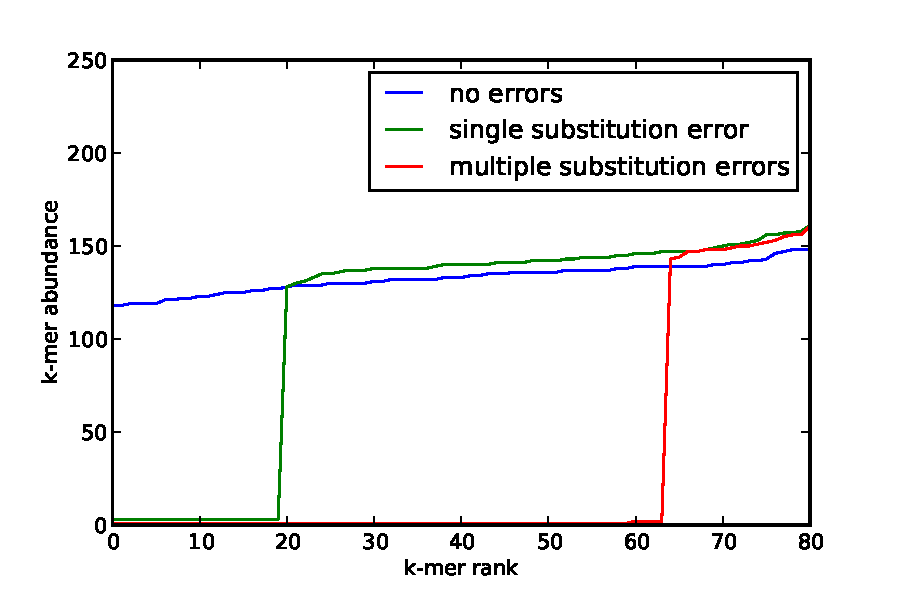
\includegraphics[width=4in]{diginorm-ranks.pdf}}
\caption{
{\bf Representative rank-abundance distributions for 20-mers from 100-base reads with no errors,
a read with a single substitution error, and a read with multiple
substitution errors.}}
\label{fig:rankabund}
\end{figure}

\begin{figure}[!ht]
\begin{center}
\centerline{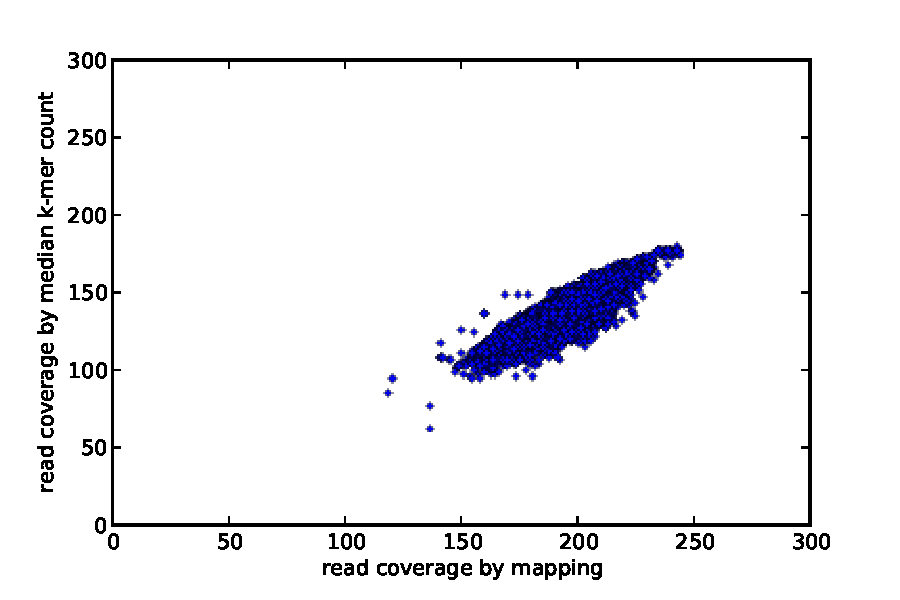
\includegraphics[width=4in]{diginorm-sim-genome.pdf}}
\centerline{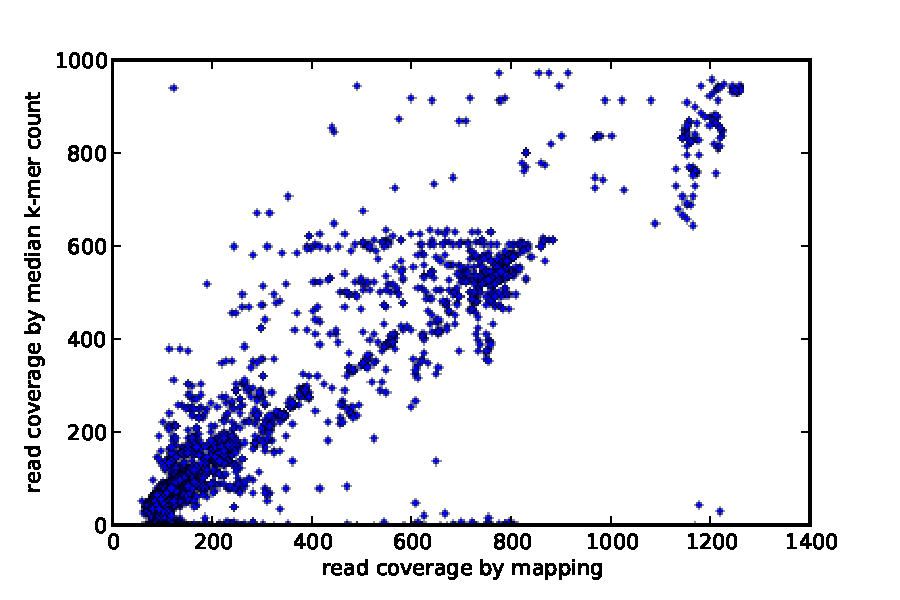
\includegraphics[width=4in]{diginorm-ecoli-genome.pdf}}
\end{center}
\caption{
{\bf Mapping and k-mer coverage measures correlate for simulated genome
data and a real {\em E. coli} data set (5m reads).  Simulated data $r^2 = 0.79$; {\em
E. coli} $r^2 = 0.80$.}
}
\label{fig:random}
\end{figure}

\begin{figure}[!ht]
\begin{center}
\centerline{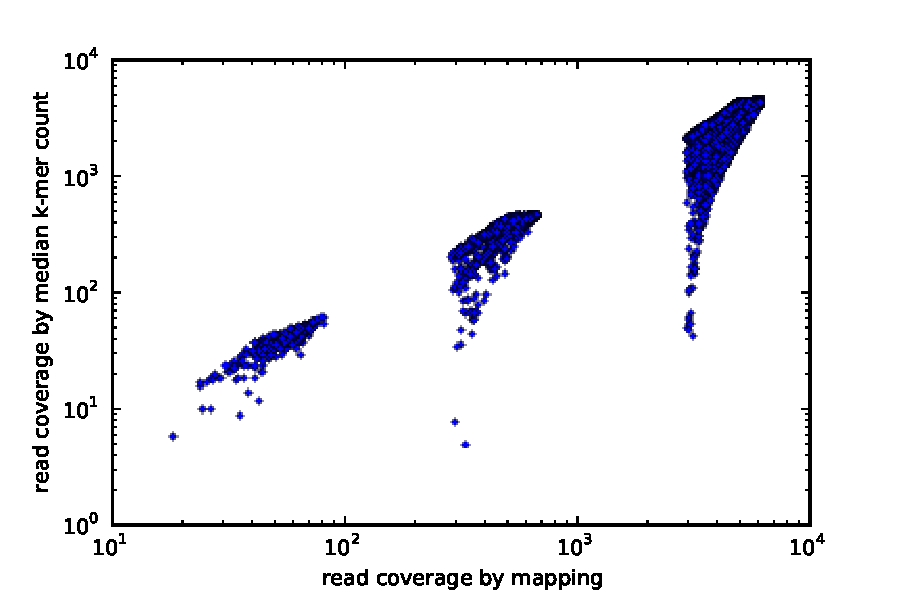
\includegraphics[width=4in]{diginorm-sim-transcr.pdf}}
\centerline{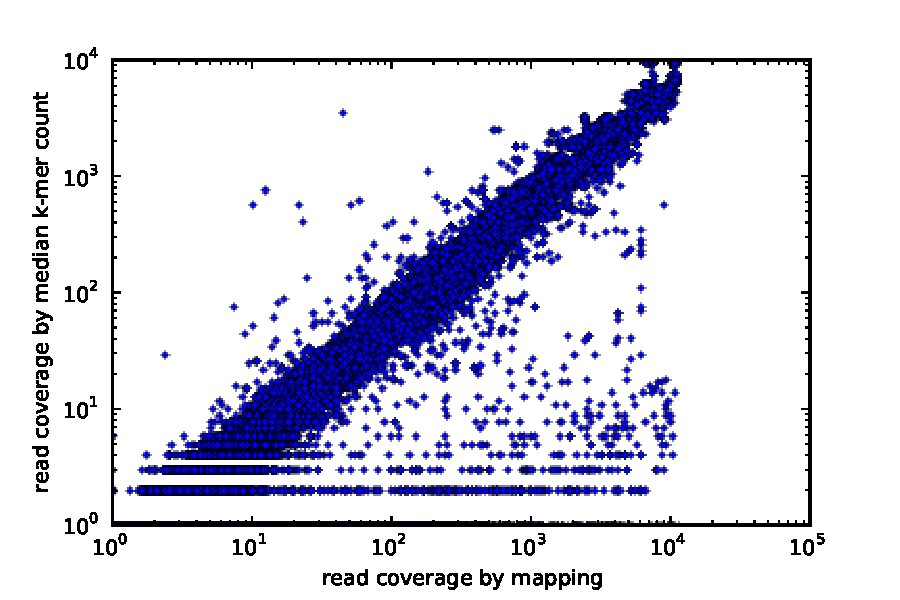
\includegraphics[width=4in]{diginorm-mouse-transcr.pdf}}
\end{center}
\caption{
{\bf Mapping and k-mer coverage measures correlate for simulated transcriptome data as well as real mouse transcriptome data. Simulated data $r^2 = 0.93$;
mouse transcriptome $r^2 = 0.90$.}
}
\label{fig:transcripts}
\end{figure}

\begin{figure}
\centerline{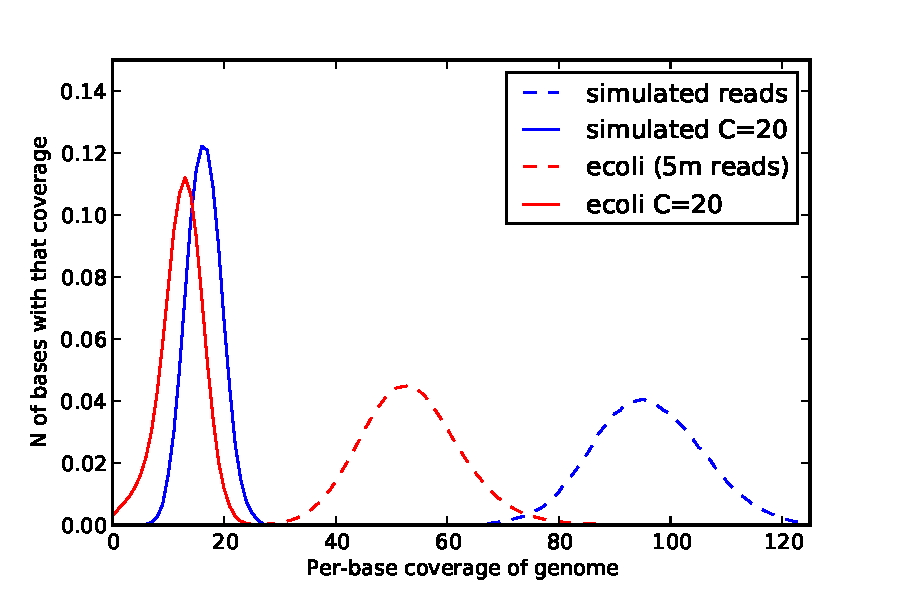
\includegraphics[width=4in]{diginorm-coverage.pdf}}
\caption{
{\bf Coverage distribution of simulated and real genomes, calculated from mapped reads before and after normalization (k=20, C=20).}}
\label{fig:coverage}
\end{figure}

\begin{figure}
\centerline{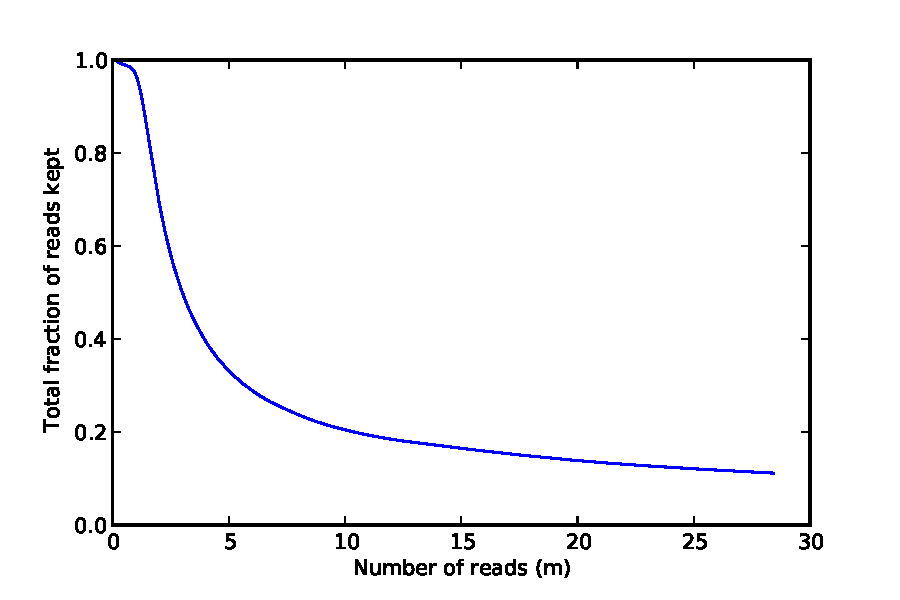
\includegraphics[width=4in]{diginorm-accumulation.pdf}}
\caption{
{\bf Fraction of reads kept when normalizing the {\em E. coli} dataset to C=20 at k=20.}}
\label{fig:accumulate}
\end{figure}

\begin{figure}
\centerline{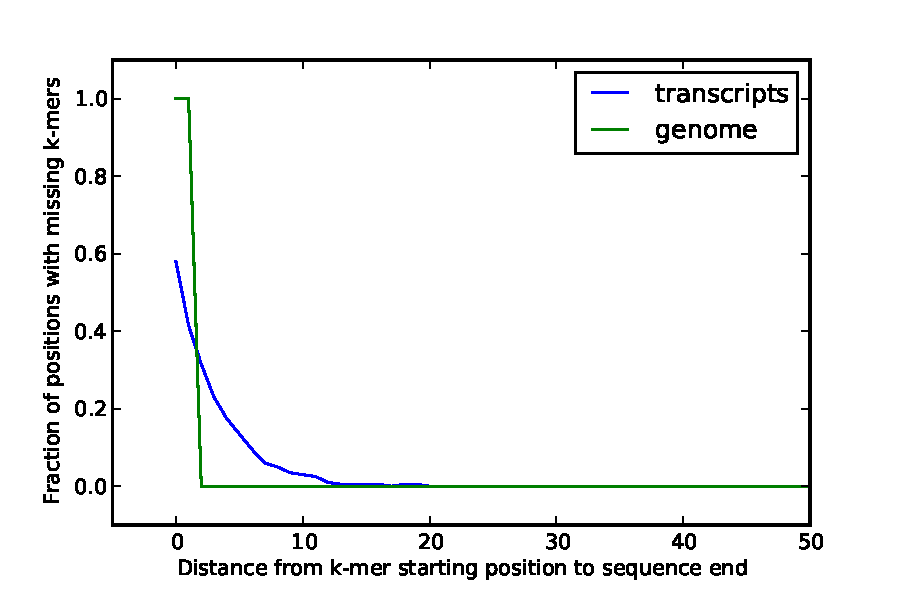
\includegraphics[width=4in]{diginorm-endbias.pdf}}
\caption{
{\bf K-mers at the ends of sequences are lost during digital normalization.}}
\label{fig:endloss}
\end{figure}

\section*{Tables}

\begin{table}[!ht]
\caption{
\bf{Digital normalization to C=20 removes many erroneous k-mers from sequencing data sets.  Numbers
in parentheses indicate number of true k-mers lost at each step, based on reference.}}
\begin{tabular}{|l|c|c|c|c|c|}
Data set & True 20-mers & 20-mers in reads & 20-mers at C=20 & \% reads kept\\
\hline \\
Simulated genome & 399,981 & 8,162,813 & 3,052,007 (-2) & 19\% \\
Simulated mRNAseq & 48,100 & 2,466,638 (-88) & 1,087,916 (-9) & 4.1\% \\
{\em E. coli} genome & 4,542,150 & 175,627,381 (-152) & 90,844,428 (-5) & 11\% \\
Yeast mRNAseq & 10,631,882 & 224,847,659 (-683) & 10,625,416 (-6,469) & 9.3\% \\
Mouse mRNAseq & 43,830,642 & 709,662,624 (-23,196) & 43,820,319 (-13,400) & 26.4\% \\
\end{tabular}
\begin{flushleft}
\end{flushleft}
\label{tab:normC20}
\end{table}

%@ note that assembly does not exactly match read k-mer content!

%%%%%%%%%%%%%%%%%

\begin{table}[!ht]
\caption{
\bf{Three-pass digital normalization removes most erroneous k-mers.  Numbers
in parentheses indicate number of true k-mers lost at each step, based on known reference.}}
\begin{tabular}{|l|c|c|c|c|}
Data set & True 20-mers & 20-mers in reads & 20-mers remaining & \% reads kept\\
\hline \\
Simulated genome & 399,981 & 8,162,813 & 453,588 (-4) & 5\% \\
Simulated mRNAseq & 48,100 & 2,466,638 (-88) & 182,855 (-351) & 1.2\% \\
{\em E. coli} genome & 4,542,150 & 175,627,381 (-152) & 7,638,175 (-23) & 2.1\% \\
Yeast mRNAseq & 10,631,882 & 224,847,659 (-683) & 10,532,451 (-99,436) & 2.1\% \\
Mouse mRNAseq & 43,830,642 & 709,662,624 (-23,196) & 42,350,127 (-1,488,380) & 7.1\% \\
\end{tabular}
\begin{flushleft}
\end{flushleft}
\label{tab:normC5}
\end{table}

%%%%%%%%%%%%%%%%%%%%%%%

\begin{table}[!ht]
\caption{
\bf{Three-pass digital normalization reduces computational requirements for contig assembly of genomic data.}}
\begin{tabular}{|l|c|c|c|c|}

Data set & N reads pre/post & Assembly time pre/post & Assembly memory pre/post \\
\hline \\
%{\em E. coli} subset & 5m / 0.4m & 235s / 24s (9.8x) & 2.7gb / 0.4gb (6.8x) \\
{\em E. coli} & 31m / 0.6m & 1040s / 63s (16.5x) & 11.2gb / 0.5 gb (22.4x) \\ 
{\em S. aureus} single-cell & 58m / 0.3m & 5352s / 35s (153x) & 54.4gb / 0.4gb (136x) \\
{\em Deltaproteobacteria} single-cell & 67m / 0.4m & 4749s / 26s (182.7x) & 52.7gb / 0.4gb (131.8x) \\

\end{tabular}
\begin{flushleft}
\end{flushleft}
\label{tab:dngenome}
\end{table}



%%%%%%%%%%%%%%%%%%

\begin{table}[!ht]
\caption{
\bf{Single-pass digital normalization to C=20 reduces computational
requirements for transcriptome assembly.}}

%add yeast

\begin{tabular}{|l|c|c|c|c|}

Data set & N reads pre/post & Assembly time pre/post & Assembly memory pre/post \\
 \hline \\
Yeast (Oases) & 100m / 9.3m & 181 min / 12 min (15.1x) & 45.2gb / 8.9gb (5.1x) \\
Yeast (Trinity) & 100m / 9.3m & 887 min / 145 min (6.1x) & 31.8gb / 10.4gb (3.1x) \\
Mouse (Oases) & 100m / 26.4m & 761 min/ 73 min (10.4x) & 116.0gb / 34.6gb (3.4x) \\
Mouse (Trinity) & 100m / 26.4m & 2297 min / 634 min (3.6x) & 42.1gb / 36.4gb (1.2x) \\
\end{tabular}

\begin{flushleft}
\end{flushleft}
\label{tab:dntrans}
\end{table}

%%%%%%%%%%%%%%%%%%%%%%%%%%%

\begin{table}[!ht]
\caption{
\bf{Digital normalization has assembler-specific effects on transcriptome
assembly.}}

%add yeast

\begin{tabular}{|l|c|c|c|c|}

Data set & Contigs $>$ 300 & Total bp $>$ 300 & Contigs $>$ 1000 & Total bp $>$ 1000 \\
\hline \\
Yeast (Oases) & 12,654 / 9,547 & 33.2mb / 27.7mb & 9,156 / 7,345 & 31.2mb / 26.4mb \\
Yeast (Trinity) & 10,344 / 12,092 & 16.2mb / 16.5mb & 5,765 / 6,053 & 13.6 mb / 13.1mb \\
Mouse (Oases) & 57,066 / 49,356 & 98.1mb / 84.9mb & 31,858 / 27,318 & 83.7mb / 72.4mb \\
Mouse (Trinity) & 50,801 / 61,242 & 79.6 mb / 78.8mb & 23,760 / 24,994 & 65.7mb / 59.4mb \\

\end{tabular}

\begin{flushleft}
\end{flushleft}
\label{tab:dntrans0}
\end{table}


\end{document}

% Candes, E.J., & Wakin, M.B., An Introduction To Compressive Sampling, IEEE Signal Processing Magazine, V.21, March 2008 [3]
